% This is samplepaper.tex, a sample chapter demonstrating the
% LLNCS macro package for Springer Computer Science proceedings;
% Version 2.20 of 2017/10/04
%
\documentclass[runningheads]{llncs}
%
\usepackage[utf8]{inputenc}
\usepackage{graphicx}
\usepackage{float}
\usepackage{caption}
% Used for displaying a sample figure. If possible, figure files should
% be included in EPS format.
%
% If you use the hyperref package, please uncomment the following line
% to display URLs in blue roman font according to Springer's eBook style:
% \renewcommand\UrlFont{\color{blue}\rmfamily}

\begin{document}
%


\title{SLIMME Vis - Interactive visual candidate exploration for SLIM}
%
%\titlerunning{Abbreviated paper title}
% If the paper title is too long for the running head, you can set
% an abbreviated paper title here
%
\author{Matthias Müller-Brockhausen; s2084740}
%
% First names are abbreviated in the running head.
% If there are more than two authors, 'et al.' is used.
%
\institute{Universiteit Leiden}
%
\maketitle              % typeset the header of the contribution
%
\begin{abstract}
In the Field of ITDM algorithms, such as SLIM, optimize compression based on the Minimum Description Length. They apply heuristics to cope with an otherwise incalculable size of options. This paper sheds some light on the effect of these heuristics by offering a website that enables the user to interactively influence the heuristics decision and directly see the effect on the achievable compression and built code table.

\keywords{Visualization \and SLIM  \and Tree \and Code Table \and Candidate Exploration}
\end{abstract}
%
%
%
\section{Introduction}
Information Theoretic Data Mining (ITDM) can seem like an overwhelming topic at first glance. Requiring good knowledge of the basics of statistics and then applying these intelligently to be able to mine \emph{any} kind of data can seem daunting to newcomers.
SLIM\cite{slim}  an ITDM  algorithm that optimizes compression by means of the Minimal Description Length (see Section \ref{sec:preliminaries}) to compress transaction data is used as an example to ease the reader into the world of ITDM.
The algorithms \emph{heuristics} build a sorted candidate list  (see Section \ref{sec:candidates}) that \textbf{determines} the achievable compression of the algorithm.

Inspired by "Seeing Theory"\cite{seeingtheory}, a website that interactively explains the basics of statistics, a web tool that allows the user to influence said \emph{heuristics} decision is implemented for this paper. To make the web tool more accessible as a stand alone tool and also more closely resemble "Seeing Theory" the SLIM algorithm and its preliminaries are also visually explained on the tools website. Furthermore studies have proven that optimized visualizations and interaction (see Section \ref{sec:learning}) helps accelerate and deepen the understanding of theoretical concepts\cite{learningvis} such as the ones required for SLIM. 

The closest work to this in the field of ITDM is  \emph{SPECTRA}\cite{spectra} which allows estimating the number of frequent item sets and comparing that estimation with the actual amount via a line graph. This however does not feature an explanation of the algorithms, or offer a lot of interactiveness besides choosing a dataset to calculate on.

The programmed tool for the paper including it's source code is available online\footnote{Demo hosted on GitHub Pages at \url{https://hizoul.github.io/slimme-vis/}}\footnote{Source code hosted on GitHub at \url{https://github.com/Hizoul/slimme-vis}}.

\section{Preliminaries}
\label{sec:preliminaries}
The following is a concise overview of the basics and terms used throughout the paper. The same content is also explained visually and interactively on the produced website.
These preliminaries try to only mention things relevant to understanding the problem statement of Section \ref{sec:problem}.
For a complete explanation on the theory behind the algorithm, the original KRIMP paper\cite{krimp} and its extension SLIM\cite{slim} are best suited as the following sections are based upon them.


SLIM works on a database \emph{D}. A database is made up of transactions \emph{t}. Each transaction is a subset of \emph{i} $t\subseteq I$. A pattern language L also consists of sets of items like a transaction.
A transaction can be summarized by item sets X, in which every single item may only occur once $X \subseteq I$. 
SLIM builds a code tables \emph{CT}. A code table is made up of item sets X on the left side accompanied by a relevant numeric value concerning the set at hand. The website displays the \emph{usage} of a set on the right hand side.

One value that is constant for a set given a database is its support. The support of a set is calculated by counting the number of transactions which contain X:

\begin{equation}
\label{eq:support}
support_D(X) = |\{t \in D | X \subseteq t\}|.
\end{equation}


The \emph{usage} of a subset is defined as:
\begin{equation}
\label{eq:usage}
usage_D(X) = |\{t \in D | X \in cover(CT,t)\}|.
\end{equation}
The usage is determined by covering the full database \emph{D}.
To cover a database take the ordered sets of a code table \emph{CT}.

\centerline{\{1, 2\} \{1\} \{2\} \{3\} \{4\}}

To cover a transaction, one starts at the left. For every set check whether it is a subset of the transaction. If so it is added to the cover, and the values within the subset are removed from the transaction. This process is repeated, until the transaction is fully covered. A cover for the example would look like this:

\centerline{Transaction: 1 2 3 4}
\centerline{Cover: \{1, 2\} \{3\} \{4\}}

Covering the database is essential for calculating the usage (Equation \ref{eq:usage}).

Since the cover of a transaction is done from left to right or top to bottom, the order of the sets of items \emph{I} is of importance!
A badly ordered list could result in a suboptimal cover:

\centerline{\{1\} \{2\} \{3\} \{4\}  \{1, 2\}}
\centerline{Transaction: 1 2 3 4}
\centerline{Cover: \{1\} \{2\} \{3\} \{4\}}
 
SLIMS uses the so called \emph{standard cover order} portrayed in Figure \ref{fig:sco}.
In words: The longest subsets should be first. Along the same length of subsets the ones with the highest support come first. If those two criteria are equal, then just sort them lexicographically.
\begin{figure}
\centerline{$|X|$ $\downarrow \quad supp_D(X)$ $\downarrow\quad$  lexicographically $\uparrow$ }
\caption{The \emph{standard cover order} used in KRIMP and SLIM to sort a code table}
\label{fig:sco}
\end{figure}

Thanks to Shannons Entropy one can convert the usage into a probability distribution:

\begin{equation}
\label{eq:probab}
P(X|D) = \frac{usage_D(X)}{\sum_{Y\in CT}usage_D(Y)}
\end{equation}

This in turn allows the assignment of a code length for each of the set in the code table \emph{CT} (more frequent = shorter code).

The individual set code lengths can be combined to calculate the required amount of bits to encode a full database \emph{D} via a code table \emph{CT}

\begin{equation}
\label{eq:codeLength}
L(D | CT) = \sum_{t\in D}{\sum_{X\in cover(CT, t)}{-log(P(X | D))}}
\end{equation}

The goal of SLIM is to minimize this code length through the Minimum Description Length (MDL):

\begin{equation}
\label{eq:mdl}
L(H) + L(D | H)
\end{equation}

$L(H)$ is the amount of bits required to represent the description / code table \emph{CT} itself. $L(D|H)$ is the amount of bits the Database can be described in / encoded with by using the code table \emph{CT}.

\subsection{Candidates}
\label{sec:candidates}
SLIM builds a list of candidate sets \emph{F}.
A candidate is a set of items, that is probably a frequent pattern. A frequent pattern is defined as a pattern which support passes a user defined \emph{minimum support threshold} (minsup).

\begin{equation}
\label{eq:minsup}
\{ X \in L | supp_D(X) \geq minsup \}
\end{equation}

Each candidate is considered in order. SLIM adds it to the code table then tests whether the code length to encode the whole database has reduced or not. If it reduced keep the candidate in the list and test the next one.

SLIM orders its candidates using the Gain Order. The gain is an approximation to the probable impact on the encoding length of the code table if the candidate were added. 

The order of the candidates is of great importance, for similar reasons as for the cover order explained in Section \ref{sec:preliminaries}.
First adding one candidate might make the second candidate not reduce the code length any more, although it could have were it added first.

To numerically determine the quality of a given code table the relative compression is used. That is the percentage of saveable bits if it is encoded with the given code table instead of the standard code table.

\begin{equation}
\label{eq:relative}
L\% = \frac{L(D, CT)}{L(D, ST)} * 100
\end{equation}

\section{Problem Statement}
\label{sec:problem}
As mentioned in Section \ref{sec:candidates} the order of the code table \emph{CT} and the order of the candidates \emph{F} make or break the found optimum of the algorithm.
With respect to runtime, it is infeasible to try out all possible orders, which is why the heuristic is needed.
The achievable relative compression is in turn determined by the order that the heuristic produces.
In the KRIMP paper, a variation called KRAMP is presented. This variant still uses the same order, but it always explores all possible paths, instead of only taking the best option.
The runtime of course rose to be impractical, but the achieved compression was \emph{slightly} better than the one of KRIMP. Meaning using alternative paths, that don't seem optimal to the heuristic can result in better code tables.
On the question of how to incorporate subjective interestingness, Tijl de Bie states:

"[...]this can only be done if the
data miner (the user) is an integral part of the analysis, considered as much as
the data and the patterns themselves. More specifically, to understand what is
interesting to a user, we will need to understand how to model the beliefs of that
user, how to contrast a pattern with this model, and how that model evolves
upon presentation of a pattern to that user"\cite{de2013subjective}

These problems are tried to be solved by providing the interactive candidate space explorer shown in Figure \ref{fig:random} and \ref{fig:customWalk}.
Every time the candidates of \emph{F} are ordered, a list of up to 10 candidates is shown together with the final compression ratio, if the candidate were added to the code table at this point in time.
The final compression ratio means, adding the candidate shown, but then just letting the SLIM algorithm finish without further user intervention.
Every candidate can be clicked to explore the next ten best candidates and further refine the candidates that influence the relative encoding.
With this functionality the user can get a better understanding of the actual effect of the orders, and by choosing himself also gets a chance to apply his previous beliefs to the outcome of the code table.
Additionally the analyst can vary the sorting between descending and ascending gain order as well as a random order to underline the effect of the order on the relative compression.


\section{Results}
\label{sec:experiment}
The following experiment is made on a small prepared dataset, which is displayed (and modifiable) within the tool.
The effect of the achievable compression (see Equation \ref{eq:relative}) already becomes clear by merely switching between the different offered sortings (namely Gain Descending, Ascending, Random).
The standard descending gain order finds its optimum at a compression rate of 30.48\%. Using a random sort however shows that the compression can go as low as 26.67\% as evident from Figure \ref{fig:random}. Since the order is random it might take a few tries of selecting the random sort to reproduce the result.
\begin{figure}
\center
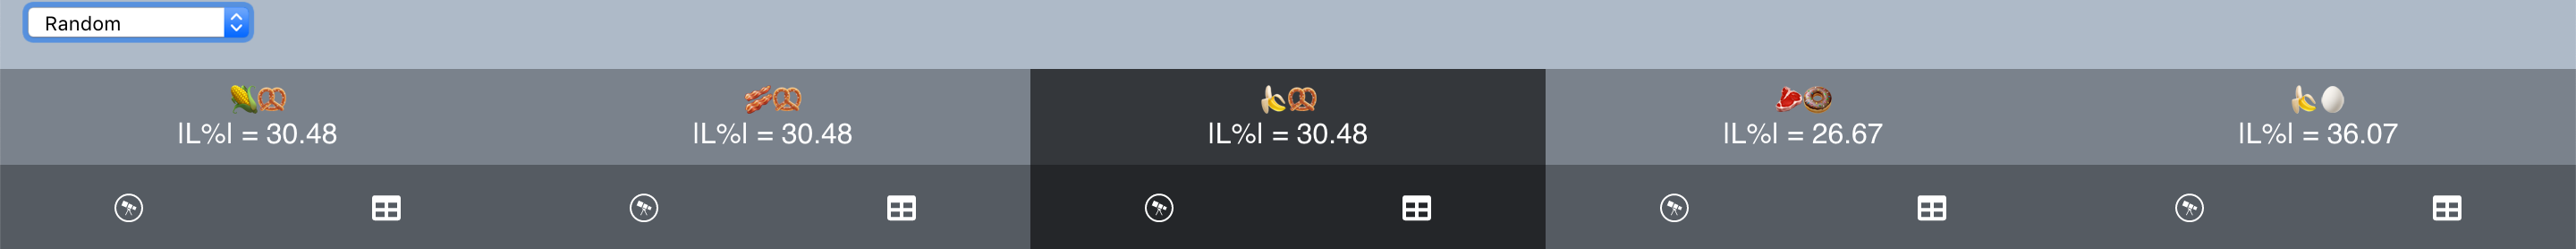
\includegraphics[width=1\linewidth]{img/random_better.png}
\caption{The candidate explorer, displaying up to 10 candidates from \emph{F}. Random sort is applied in this instance.}
\label{fig:random}
\end{figure}

Manually exploring within the descending gain order, as shown in Figure \ref{fig:customWalk}, reveals that one has to use options that wouldn't be considered by the heuristic multiple times in order to achieve a compression of 26.67\%.
The ascending gain order, as to be expected, delivers the worst result with 63.35\%. With random similarly bad results are possible.

\begin{figure}
\center
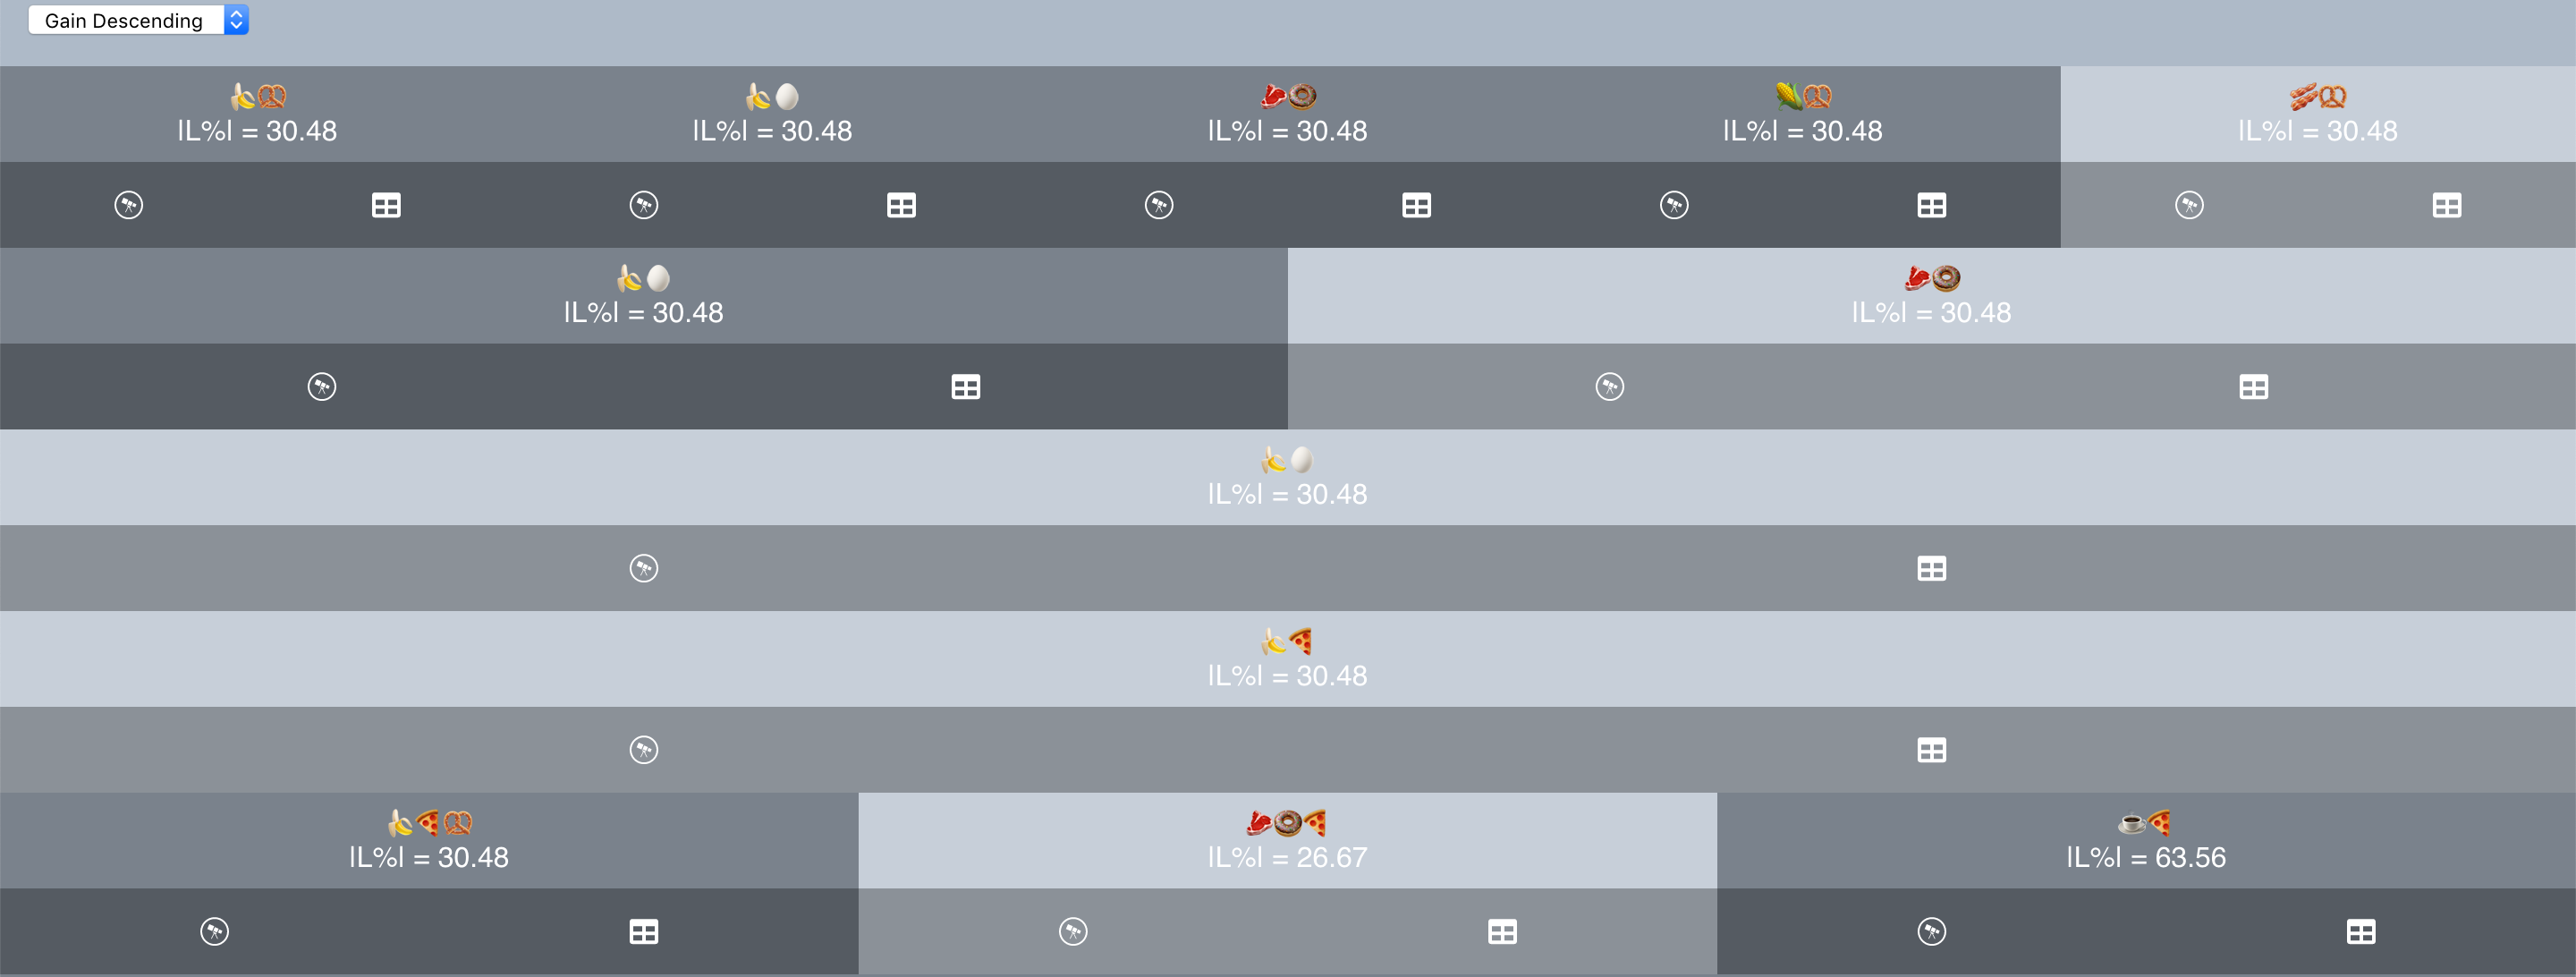
\includegraphics[width=1\linewidth]{img/custom_walk.png}
\caption{The candidate explorer, displaying up to 10 candidates from \emph{F}. The standard descending gain order is applied, and a custom path chosen to reproduce the achieved compression of a lucky random exploration displayed in Figure \ref{fig:random}.}
\label{fig:customWalk}
\end{figure}
\section{Discussion}
\subsection{Algorithm}
\label{sec:insights}

A problem encountered during implementation was that, that the post-prune mechanism does not verify if the code table is still valid.
Some relative compressions were so good that they seemed to good to be true. And in fact they were because they could not fully cover every transaction of the database. Furthermore an endless loop of pruning and then re-adding the same pair over and over could happen.
To solve this problem, the post-prune mechanism was extended to check, whether removing a set from the code table renders it invalid. Only if it is still valid the item will actually be pruned.

The implemented candidate exploration tool also offers some room for improvement.
It would for example be beneficial for processing larger datasets if a specific pattern could be specified and the candidate space exploration only starts as soon as that specific pattern is reached.
Without such a functionality it could be a very slow process to model the users belief onto a large dataset.
Similar to that one could also say, do x iterations of SLIM and from that state on forward let me do the interactive candidate exploration.

\subsection{Maximizing Learning Efficiency}
\label{sec:learning}
As this paper is providing an explanatory website for the basics required for SLIM, it is relevant to assess the possibilities this offers in contrast to a traditional scientific paper.
The field of psychology has long known, that there are certain features, our brain can process without any sort of focus via our subconsciousness.
Some of the most prominently known \emph{preattentive features} are color, orientation\cite{healey1996high} and shape\cite{treisman1988feature}.
In 1993 Janiszewski has shown, that by implementing these preattentive features into advertisements, the probability that people subconciously remember a brand name while scanning through a newspaper is increased\cite{janiszewski1993preattentive}.
An interesting aspect of these preattentive features is that they can be processed in parallel, similar to multithreading on a computer, which makes it easier for people skimming through a document to see relevant parts\cite{healey1996high}.
However it is important to note, that using too many preattentive features at once, can actually decrease the subjects unconcious processing, and requires more manual focus\cite{wolfe1992parallel}.
Building upon this knowledge, every variable introduced in the preliminaries Section \ref{sec:preliminaries} (e.g. transaction \emph{t}) is associated to a specific color and icon. An example of this can be seen in Figure \ref{fig:colors}.

Furthermore for every item \emph{i} that occurs in the sets of transactions and code tables, a \emph{translation} is used to translate the item id into a shape. That way while exploring possible candidates the user can more quickly recognize a path of items he would like to follow.


\begin{figure}[H]
\center
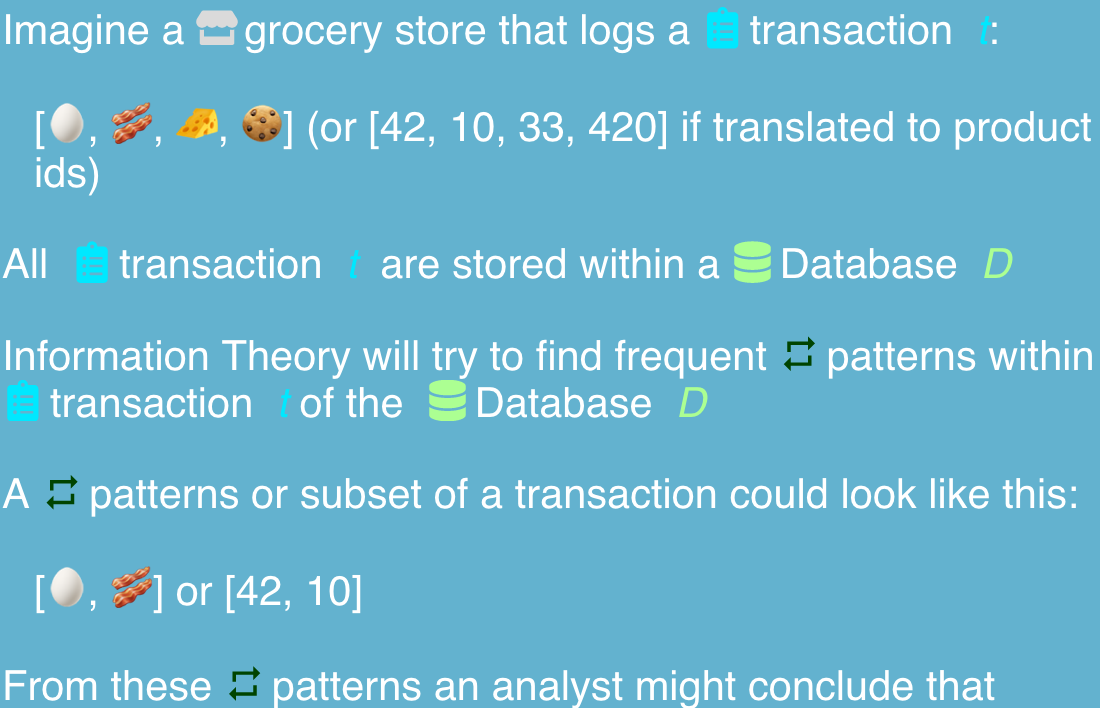
\includegraphics[width=1\linewidth]{img/color_coding.png}
\caption{An example of color coding keywords in the explanation to enhance recognizability.}
\label{fig:colors}
\end{figure}
\section{Conclusion}
An interactive learning experience, optimized for learning efficiency (Section \ref{sec:learning}), has been created to ease the user into the world of ITDM at the example of SLIM.
Furthermore the candidate space exploration of SLIM has been made interactive and now allows the analyst to influence the result according to his beliefs (Section \ref{sec:problem}). Section \ref{sec:experiment} underlined how the default heuristic used in SLIM only produces a local optimum. This was proven by showing that the default sort finds a relative compressiomn of 30.48\% whereas a manual exploration and also a completely random one can achieve up to 26.67\%.
Additionally for people that wish to reimplement and play around with SLIM, further details relevant for a working implementation are shared in Section \ref{sec:insights}.

%
% ---- Bibliography ----
%
% BibTeX users should specify bibliography style 'splncs04'.
% References will then be sorted and formatted in the correct style.
%
\bibliographystyle{splncs04}
\bibliography{report}
%
\end{document}
